% PDR paper draft (TASKS.md T12). Every number comes from numbers.tex, which
% scripts/make_figures.py generates from docs/claims.json (recomputed from raw
% data by scripts/check_claims.py). Do not type numbers by hand.
\documentclass[conference]{IEEEtran}
\IEEEoverridecommandlockouts
% Layout follows the Overleaf "IEEE Conference Template" (IEEEtran, conference mode).
\usepackage{cite}
\usepackage{textcomp}
\def\BibTeX{{\rm B\kern-.05em{\sc i\kern-.025em b}\kern-.08em
    T\kern-.1667em\lower.7ex\hbox{E}\kern-.125emX}}
\usepackage{graphicx}
\usepackage{booktabs}
\usepackage{amsmath}
\usepackage{url}
\usepackage{xcolor}
% generated by scripts/make_figures.py from docs/claims.json -- do not edit
\newcommand{\POneRepos}{45}
\newcommand{\POneEdges}{69,692}
\newcommand{\POneUnknown}{1.09}
\newcommand{\POneOPG}{83.29}
\newcommand{\POneOPGci}{[79.3, 87.0]}
\newcommand{\POneOPGrepo}{81.3}
\newcommand{\POneOPGrepoCi}{[77.9, 84.8]}
\newcommand{\POneDeficient}{57,415}
\newcommand{\POneProxy}{2,349}
\newcommand{\POneProxyPct}{4.09}
\newcommand{\POneProxyCi}{[2.0, 6.3]}
\newcommand{\POneProxyRepo}{2.7}
\newcommand{\POneProxyRepoCi}{[1.6, 3.9]}
\newcommand{\LOneOK}{638}
\newcommand{\LOneN}{2,349}
\newcommand{\LOneRipple}{1,656}
\newcommand{\LOnePeer}{55}
\newcommand{\LOnePct}{27.16}
\newcommand{\LOneCi}{[18.0, 40.1]}
\newcommand{\LOneRepo}{52.3}
\newcommand{\LOneRepoCi}{[41.5, 63.0]}
\newcommand{\AltExists}{27.67}
\newcommand{\AltExistsCi}{[18.2, 41.5]}
\newcommand{\AltExistsRepo}{52.7}
\newcommand{\AltRecovered}{12}
\newcommand{\AltPop}{1,711}
\newcommand{\AltNoAlt}{524}
\newcommand{\AltBlocked}{384}
\newcommand{\RipOne}{41.42}
\newcommand{\RipOneRepo}{65.1}
\newcommand{\RipFive}{63.60}
\newcommand{\RipFiveRepo}{80.7}
\newcommand{\LTwoN}{13}
\newcommand{\LTwoOK}{13}
\newcommand{\MPOK}{12}
\newcommand{\MPInvalid}{11}
\newcommand{\MPN}{23}
\newcommand{\MPJudge}{12}
\newcommand{\SRepos}{160}
\newcommand{\SEdges}{262,066}
\newcommand{\SUnknown}{1.94}
\newcommand{\SOPG}{84.80}
\newcommand{\SOPGci}{[82.7, 87.0]}
\newcommand{\SOPGrepo}{83.4}
\newcommand{\SOPGrepoCi}{[80.8, 85.8]}
\newcommand{\SDeficient}{217,924}
\newcommand{\SProxy}{17,549}
\newcommand{\SProxyPct}{8.05}
\newcommand{\SProxyCi}{[6.7, 9.4]}
\newcommand{\SProxyRepo}{5.8}
\newcommand{\SProxyRepoCi}{[4.7, 7.0]}
\newcommand{\SLOK}{5,003}
\newcommand{\SLPct}{28.51}
\newcommand{\SLCi}{[23.8, 33.3]}
\newcommand{\SLRepo}{45.2}
\newcommand{\SLRepoCi}{[39.8, 50.8]}
\newcommand{\SLRipple}{10,860}
\newcommand{\SLPeer}{1,573}
\newcommand{\SLFail}{113}
\newcommand{\SEndToEnd}{2.30}
\newcommand{\SScreened}{91}
\newcommand{\STestable}{31}
\newcommand{\STestablePct}{34.1}
\newcommand{\STestableCi}{[25.2, 44.3]}
\newcommand{\SExp}{110}
\newcommand{\SJudge}{108}
\newcommand{\SJudgeRepos}{30}
\newcommand{\SOK}{97}
\newcommand{\SLifecycle}{12}
\newcommand{\STestFail}{1}
\newcommand{\SOKJudgePct}{88.89}
\newcommand{\SOKJudgeCi}{[75.5, 100.0]}
\newcommand{\SNewTest}{0}
\newcommand{\SPairsTest}{108}
\newcommand{\SNewInstall}{0}
\newcommand{\SNewLifecycle}{0}
\newcommand{\SPairsInstall}{110}
\newcommand{\SRuleThree}{2.8}
\newcommand{\SRuleThreeRepo}{10}
\newcommand{\SGainPos}{99}
\newcommand{\SGainN}{110}

\newcommand{\todo}[1]{\textcolor{red}{[TODO: #1]}}

\begin{document}

\title{Missing Provenance at Resolution Time:\\A Consumer-Side Study of How Much\\npm Version Choice Can Recover}

\author{\IEEEauthorblockN{Aakash G S}
\IEEEauthorblockA{\textit{Department of Computer Science and Business Systems} \
\textit{SRM Institute of Science and Technology}\
Chennai, India \
ag5901@srmist.edu.in}
\and
\IEEEauthorblockN{Hariharan J P}
\IEEEauthorblockA{\textit{Department of Computer Science and Business Systems} \
\textit{SRM Institute of Science and Technology}\
Chennai, India \
hj0956@srmist.edu.in}
\and
\IEEEauthorblockN{Jaswanth Raj}
\IEEEauthorblockA{\textit{Department of Computer Science and Business Systems} \
\textit{SRM Institute of Science and Technology}\
Chennai, India \
jj3494@srmist.edu.in}
}

\maketitle

\begin{abstract}
npm can attach build provenance to published package versions, and tools now
let projects require it. Recent release-side measurement asks how each release
reached the registry; we study the other end of the supply chain, the
consumer at resolution time. We ask a practical question: when a resolved
dependency lacks provenance, can a project recover it by choosing a different
version inside the range it already declares, and what does that cost? On
\SRepos{} randomly sampled, commit-pinned open-source repositories
(\SEdges{} resolved dependency edges) we measure a funnel with attrition at
every stage. \SOPG\% of edges lack provenance; only \SProxyPct\% of those have
an in-range provenance-bearing version within a minor/patch step of what is
resolved; and only \SLPct\% of those (repository-clustered 95\% CI \SLCi) are
accepted by npm's own resolver without changing any other package. End to end,
\SEndToEnd\% of deficient edges are recoverable this way. Once a candidate passes
the resolver, however, switching to it caused no attributable failure in
installation, lifecycle scripts, peer dependencies, signature audit, or the
repository's own tests in any of \SExp{} isolated experiments across
\STestable{} repositories with reproducible test suites. The limiting factor is
the availability of provenance-bearing versions and their acceptance by the
resolver, not breakage. All data, pre-registration tags and analysis code are
public.
\end{abstract}

\begin{IEEEkeywords}
software supply chain, npm, build provenance, dependency resolution, consumer-side, empirical study
\end{IEEEkeywords}

\section{Introduction}

Software supply-chain attacks on package registries have made the origin of a
package version a first-class question. npm provenance records, as a signed
attestation, the source repository and build that produced a published
version~\cite{npmprovenance2023}. Provenance is \emph{origin evidence}; it is
not a statement that a package is safe, and we never use it as one.

Most measurement of this evidence is \emph{producer-side}: it looks at
releases as they are published. Santos-Grueiro~\cite{santos2026authority}
compares each release with its immediate predecessor across publisher,
repository, workflow, provenance and signing evidence in five registries, and
turns public release-path discontinuities, including provenance
disappearance, into a release-time review queue. That work deliberately sets
dependency graphs aside as describing consumption rather than production, so
it does not ask what a \emph{consumer} can do. A project does not choose
releases one at a time; it declares ranges and lets a resolver pick a whole
tree. This paper is a \emph{consumer-side, resolution-time} study. Our unit is
a resolved dependency edge in a real application lockfile, and our question is
how much origin evidence that project can obtain through the version choices
its own declared ranges and npm's resolver allow.

Registries and package managers are beginning to let consumers require such
evidence. A project that enables such a policy will find that most of its
resolved dependencies lack provenance. The natural remedy is version choice:
pick, within the semantic-versioning range each dependency already declares,
a version that carries provenance. Whether this works in practice depends on
three things that are easy to assume and hard to know: whether such versions
exist, whether npm's real resolver accepts them without disturbing the rest
of the tree, and whether the project still installs and passes its tests.

We measure all three. Our contributions are:
\begin{itemize}
\item A consumer-side, resolution-time view of provenance that complements
  release-side measurement~\cite{santos2026authority}: we measure origin
  evidence where a project actually acquires it, on resolved lockfile edges,
  under its own declared ranges and npm's real resolver.
\item A funnel measurement of provenance recoverability on two corpora
  (\POneRepos{} and \SRepos{} repositories), separating availability, resolver
  acceptance, and behaviour, with edge- and repository-weighted estimates and
  repository-clustered confidence intervals.
\item An isolated execution harness (disposable containers, an
  allowlisting network proxy, a verified network self-test) that runs real
  installs, lifecycle scripts and test suites of untrusted packages for both
  the original and the substituted dependency tree.
\item Evidence that the binding constraint is availability and resolution:
  the resolver rejects most screening-positive candidates, lower
  provenance-bearing versions almost never help, and resolver-accepted
  substitutions showed no attributable behavioural failures.
\item A public, pre-registered artifact in which every number in this paper
  is recomputed from raw data by a test.
\end{itemize}

\section{Research Questions}
\textbf{RQ1} How many resolved dependency edges lack provenance?
\textbf{RQ2} How many deficient edges have an in-range provenance-bearing
candidate, and how many does npm's resolver accept (single best candidate and
any candidate)?
\textbf{RQ3} Among resolver-accepted substitutions, how many keep the project
installable, its lifecycle scripts and peer dependencies intact, its audit
signature status, and its own tests passing?
\textbf{RQ4} How sensitive are these answers to the definition of ``without
disturbing the tree''?

\section{Method}

\subsection{Corpora}
\emph{Phase~1} covers \POneRepos{} well-known JavaScript projects with a
committed lockfile (\POneEdges{} edges), selected in an earlier pilot.
\emph{scale\_v1} is a stratified random sample designed and frozen in
version control before any data were fetched: from a frame of public GitHub
repositories in JavaScript or TypeScript with at least 1,000 stars, active
in the last six months, we drew 20 repositories in each of eight strata
(four star bands $\times$ created before/after 2018) that have a root
\texttt{package-lock.json} (lockfile version $\geq 2$). Each repository is
pinned to the commit it was sampled at.

\subsection{Classification (RQ1, RQ2)}
We parse every lockfile into dependency edges (requester, declared range,
resolved version). A version has provenance iff its registry metadata carries
\texttt{dist.attestations}. An edge is \emph{deficient} if its resolved version
lacks provenance and \emph{screening-positive} if the highest
provenance-bearing version satisfying the declared range differs from the
resolved one by at most a minor or patch step. All range logic uses npm's own
\texttt{semver} library.

\subsection{Resolver confirmation, Layer 1 (RQ2, RQ4)}
For each screening-positive edge we force the candidate with an
\texttt{overrides} entry (or by editing the direct dependency when the package
is a root dependency, which \texttt{overrides} rejects) and re-resolve with
\texttt{npm install --package-lock-only --ignore-scripts}, npm 10.9.7. A
candidate is \emph{OK} if it is applied and no other top-level package changes
version; otherwise \emph{RIPPLE}, or \emph{PEER\_CONFLICT} on
\texttt{ERESOLVE}. Nothing executes. A pre-registered follow-up experiment tried up to five lower
provenance-bearing in-range versions for every non-OK edge.

\subsection{Behaviour, Layer 3 (RQ3)}
Untrusted package code runs only in a disposable container per arm: no Linux
capabilities, read-only root filesystem, non-root user, memory, CPU and
process limits, the repository snapshot mounted read-only, and an internal
network whose only exit is a proxy that admits the npm registry and Sigstore
hosts and refuses all others. A network self-test (allowed hosts reachable,
others refused and logged, direct egress impossible) must pass before any
experiment. For each experiment we run the unmodified repository (B0) and
the substituted one (PDR) through install, lifecycle scripts, a peer check,
\texttt{npm audit signatures}, and the repository's own tests, twice per arm.
The PDR arm restores the original \texttt{package.json} before testing so the
repository's own linters do not react to our edit. A failure is
\emph{attributable} only if B0 passed the same stage. In scale\_v1, a
baseline screen first ran B0 alone and only repositories whose own tests
passed twice proceeded.

\subsection{Statistics and pre-registration}
Edges within a repository are not independent. Every rate is reported
edge-weighted and repository-weighted, each with a 95\% repository-clustered
percentile bootstrap (5,000 resamples, fixed seed); repository-level
proportions use Wilson intervals. Designs, cohorts and analysis scripts were
committed and tagged before the runs they govern; changes were made only as
dated amendments with reasons stated before outcomes.

\section{Results}

\begin{figure}[t]
\centering
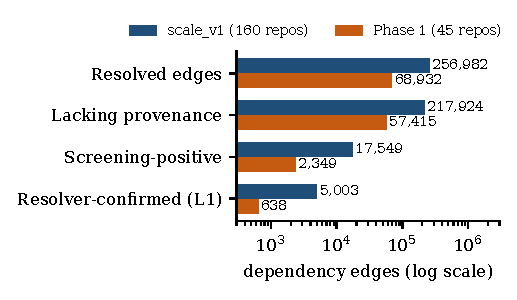
\includegraphics[width=\columnwidth]{figures/fig_funnel.pdf}
\caption{Attrition from resolved edges to resolver-confirmed recoverable edges
(log scale) in both corpora.}
\label{fig:funnel}
\end{figure}

\begin{figure}[t]
\centering
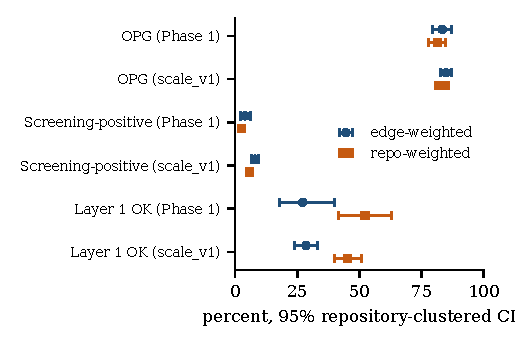
\includegraphics[width=\columnwidth]{figures/fig_forest.pdf}
\caption{Edge- and repository-weighted rates with 95\% repository-clustered CIs.
Screening-positive is among deficient edges; Layer~1 OK is among
screening-positive edges.}
\label{fig:forest}
\end{figure}

\subsection{RQ1: Most resolved edges lack provenance}
In scale\_v1, \SOPG\% of known edges lack provenance (CI \SOPGci;
repository-weighted \SOPGrepo\%, \SOPGrepoCi). Phase~1 gives \POneOPG\%
(\POneOPGci). Unknown status is below 2\% in both corpora.

\subsection{RQ2: Few candidates exist, and the resolver rejects most}
Only \SProxyPct\% of deficient edges in scale\_v1 have a screening-positive
candidate (\SProxyCi; repository-weighted \SProxyRepo\%), and \POneProxyPct\%
in Phase~1. Forcing the candidate through npm's resolver confirms
\SLPct\% of them in scale\_v1 (\SLCi; repository-weighted \SLRepo\%,
\SLRepoCi) and \LOnePct\% in Phase~1 (\LOneCi; repository-weighted \LOneRepo\%).
Table~\ref{tab:l1} shows that rejection is overwhelmingly a \emph{ripple}: the
candidate applies, but other packages move. End to end, \SEndToEnd\% of deficient
edges in scale\_v1 are recoverable by version choice without disturbing the
tree. Edge- and repository-weighted figures diverge; in Phase~1 this is because a
few repositories contribute many near-identical candidates
(Fig.~\ref{fig:forest}).

Trying lower versions barely helps. For the \AltPop{} Phase~1 edges whose
best candidate failed, up to five lower provenance-bearing in-range versions
recovered \AltRecovered{}; the exists-any rate is \AltExists\% (\AltExistsCi)
against \LOnePct\% for the single best candidate. \AltNoAlt{} of those edges had
no lower candidate at all, and \AltBlocked{} could not be evaluated on the
analysis host (reported as a bound).

\begin{table}[t]
\centering
\caption{Layer 1 outcomes (screening-positive edges).}
\label{tab:l1}
\begin{tabular}{lrr}
\toprule
Layer 1 outcome & Phase 1 & scale\_v1 \\
\midrule
\texttt{OK} & 638 & 5,003 \\
\texttt{RIPPLE} & 1,656 & 10,860 \\
\texttt{PEER\_CONFLICT} & 55 & 1,573 \\
\texttt{RESOLUTION\_FAIL} & 0 & 113 \\
Total & 2,349 & 17,549 \\
\bottomrule
\end{tabular}

\end{table}

\subsection{RQ3: Accepted substitutions behaved like the baseline}
In scale\_v1, \STestable{} of \SScreened{} repositories (\STestablePct\%, Wilson
\STestableCi) had a test suite that installed and passed twice in the isolated
worker. Across their \SExp{} experiments, no failure at any stage was
attributable to the substitution: paired failure deltas were zero for
installation (\SNewInstall{} of \SPairsInstall{} pairs), lifecycle scripts
(\SNewLifecycle{}) and tests (\SNewTest{} of \SPairsTest{}). The
\SLifecycle{} non-OK lifecycle outcomes occurred identically in the unmodified
baseline (blocked post-install downloads, a vendored binary build). With zero
events, a rule-of-three upper bound is about \SRuleThree\% per experiment and
\SRuleThreeRepo\% per repository. Audit signature status never got worse, and
\SGainPos{} of \SGainN{} substitutions increased the number of verified
attestations, as intended. Table~\ref{tab:l3} also reports the three rounds
of a pre-registered 23-experiment micro-pilot that preceded the scale-up; its
final round gave \MPOK{} OK of \MPJudge{} judgeable experiments, with
\MPInvalid{} of \MPN{} baselines unusable.

\begin{table}[t]
\centering
\caption{Layer 3 outcomes. MP = micro-pilot rounds (environment fixes between
rounds were baseline-only and pre-registered). $^\dagger$scale\_v1 screened
baselines first and ran only testable repositories.}
\label{tab:l3}
\begin{tabular}{lrrrr}
\toprule
Outcome & MP v1 & MP v2 & MP v3 & scale\_v1 \\
\midrule
\texttt{OK} & 9 & 8 & 12 & 97 \\
\texttt{TEST\_FAIL} & 12 & 12 & 6 & 1 \\
\texttt{TEST\_FLAKY} & 1 & 0 & 0 & 0 \\
\texttt{TIMEOUT} & 0 & 2 & 4 & 0 \\
\texttt{LIFECYCLE\_FAIL} & 0 & 0 & 0 & 12 \\
\texttt{INSTALL\_FAIL} & 1 & 1 & 1 & 0 \\
\midrule
Invalid baselines & 13 & 13 & 11 & 60 of 91 repos$^\dagger$ \\
Experiments & 23 & 23 & 23 & 110 \\
\bottomrule
\end{tabular}

\end{table}

\subsection{RQ4: The definition of ``undisturbed'' matters}
Layer~1's \emph{OK} allows zero other packages to change. Allowing one raises
the Phase~1 rate from \LOnePct\% to \RipOne\% (repository-weighted \RipOneRepo\%);
allowing five raises it to \RipFive\% (\RipFiveRepo\%) (Fig.~\ref{fig:ripple}).
Our headline figures use the strictest definition, so they are lower bounds on
what a project willing to accept small side effects could recover.

\begin{figure}[t]
\centering
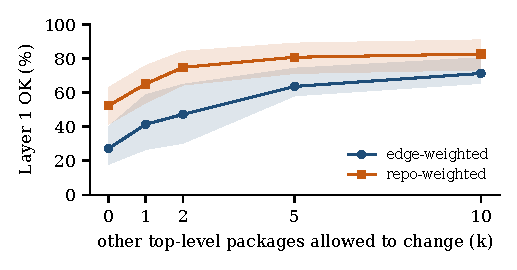
\includegraphics[width=\columnwidth]{figures/fig_ripple.pdf}
\caption{Phase~1 Layer~1 OK rate when up to $k$ other top-level packages may
change version (sensitivity analysis; $k=0$ is the frozen definition).}
\label{fig:ripple}
\end{figure}

\section{Discussion}
The funnel locates the problem. Provenance is missing for most edges, and for
over nine in ten deficient edges no provenance-bearing version exists close
to what is resolved. Where one exists, npm usually cannot adopt it in
isolation, because adopting it moves other packages. Where npm can adopt
it, we observed no behavioural cost. For maintainers this means enforcing
provenance today mostly fails for lack of supply, not because switching
breaks projects; for registry and tool designers it means the leverage is
upstream (publishers adopting provenance) and in resolution (letting a
resolver optimise for provenance rather than forcing single candidates). A
configurable solver such as MaxNPM~\cite{pinckney2023maxnpm} could find
combinations npm's resolver does not; we measured npm's own behaviour and do
not claim that better solutions are impossible.
The two ends of the supply chain also compose. A release-side trigger such as
provenance disappearance~\cite{santos2026authority} tells a reviewer that a
release path changed; at resolution time the same event appears as a
deficient edge, and our funnel says whether the consuming project could have
stayed on a provenance-bearing version without disturbing its tree. Neither
view substitutes for the other.

\section{Threats to Validity}
\emph{Construct.} Provenance presence is read from the registry's current
metadata, not at publish time. Tests measure what each project chose to test.
\emph{Internal.} Layer~3 covers only repositories whose own tests were
reproducible in a locked-down worker (\STestablePct\% of eligible ones);
projects needing network services, browsers or specific toolchains are not
represented. Single-run test outcomes can be unstable~\cite{maksymiuk2026reproducible};
we ran every arm twice and excluded flaky pairs. Our edit of
\texttt{package.json} initially caused lint failures that looked like
regressions; we found and removed this artifact before the scale-up.
\emph{External.} Both corpora are popular, actively maintained GitHub
projects with committed lockfiles; results may not hold for the long tail of
the registry or for other ecosystems. Provenance-bearing versions come from
projects whose practices may differ systematically from others~\cite{solarin2026verifiability}.
\emph{Conclusion.} With zero observed attributable failures, Layer~3 bounds
the failure rate rather than estimating it.

\section{Related Work}
Studies of npm updates measure how new versions propagate through semantic
versioning ranges~\cite{pinckney2023semver}, how often non-major updates break
clients~\cite{venturini2023broke}, how dependency bots and their
compatibility signals are used~\cite{he2023dependabot,rombaut2024crowd}, and
how other projects' tests can expose breaking versions~\cite{mujahid2020tests};
BUMP provides reproducible breaking updates for Maven~\cite{reyes2024bump}.
He, Vasilescu and K\"astner simulate npm resolution counterfactually to show
that pinning alone does not prevent supply-chain exposure~\cite{he2025pinning},
and peer-dependency conflicts can trap the resolver~\cite{wang2025peerspin}.
On origin evidence, signing adoption has been measured in four registries
other than npm~\cite{schorlemmer2024signing}, and artifact verifiability
including npm provenance~\cite{solarin2026verifiability}. Closest in subject
is Santos-Grueiro's release-authority study~\cite{santos2026authority}. For
45,812 releases in npm, PyPI, Maven Central, crates.io and RubyGems (3,427 of
them npm), it reconstructs a predecessor-aware record of publisher,
repository, workflow, provenance, signing and mediation evidence and finds 204
policy-triggering release-path discontinuities that form a bounded review
queue. Its unit is a package release compared with the previous release of
the same package, from a purposefully sampled registry cohort; its user is a
reviewer deciding whether a new release needs attention. Our unit is a
resolved dependency edge in a sampled application, and our user is the
project that must live with npm's resolution. The studies answer different
questions and their rates are not comparable: their npm provenance visibility
is a share of sampled releases, ours a share of resolved edges. They share one
signal, provenance loss between adjacent releases, which that study uses as a
review trigger and which we observe downstream as deficiency.
In the corpus we searched, no directly matching work was identified that
measures, on real application lockfiles, whether provenance-bearing versions
exist within declared ranges and how much of that apparent recovery survives
npm's resolver, installation and the project's own tests.

\section{Conclusion}
Seen from the consumer at resolution time, version choice recovers provenance
for only about \SEndToEnd\% of deficient dependency edges in our sample, almost entirely because suitable versions are
missing or the resolver cannot adopt them without side effects. When it can,
the switch did not break the projects we could test. Raising provenance
coverage is therefore mainly a question of publisher adoption and
provenance-aware resolution.

\section*{Data Availability}
Code, data, pre-registration tags and the claims registry are available at
\url{https://github.com/ftaakash/PDR}.

\section*{Acknowledgment}
The authors used Claude (Anthropic) to help build the data-collection and
analysis pipeline. All code, data and results were reviewed and verified by
the authors.

\bibliographystyle{IEEEtran}
\bibliography{refs}

\end{document}
